\section*{Аннотация}
\addcontentsline{toc}{section}{Аннотация}

Холодные нейтральные атомы в массивах оптических пинцетов являются одной из лидирующих платформ для реализации квантового компьютера. На базе данной платформы в мире уже продемонстрировано 48 логических кубитов \cite{Bluvstein:2024aa}. Для практического использования такого компьютера важно уметь выполнять однокубитные и многокубитные логические операции с высокой точностью. В работе исследуются подходы к улучшению точности однокубитных логических операций с рамановским двухфотонным возбуждением и двухкубитных логических операций, реализуемых с помощью эффекта ридберговской блокады. Проводится моделирование основных источников ошибок, включающих в себя тепловое движение атома в оптическом пинцете, спонтанный распад из промежуточного состояния, фазовые шумы лазера, ошибки приготовления и измерения состояния. Параметры модели были экспериментально измерены, что позволило выполнить моделирование без свободных параметров. Для однокубитных операций предлагается использование импульсной последовательности BroadBand 1 (BB1) \cite{WIMPERIS199046,WIMPERIS1989509,Wimperis1994BroadbandNA}, устойчивой к тепловому движению атома, амплитудным шумам лазера, неоднородностям интенсивности лазера по атомному массиву. Проводится её моделирование и обсуждаются предварительные экспериментальные результаты. Также экспериментально демонстрируется повышение точности возбуждения в ридберговское состояние, использующееся для двухкубитных логических операций, за счёт использования flat-top пучков, имеющих плоское распределением интенсивности в фокальной плоскости. 

% \vspace{2em}
\begin{figure}[ht]
	\centering
	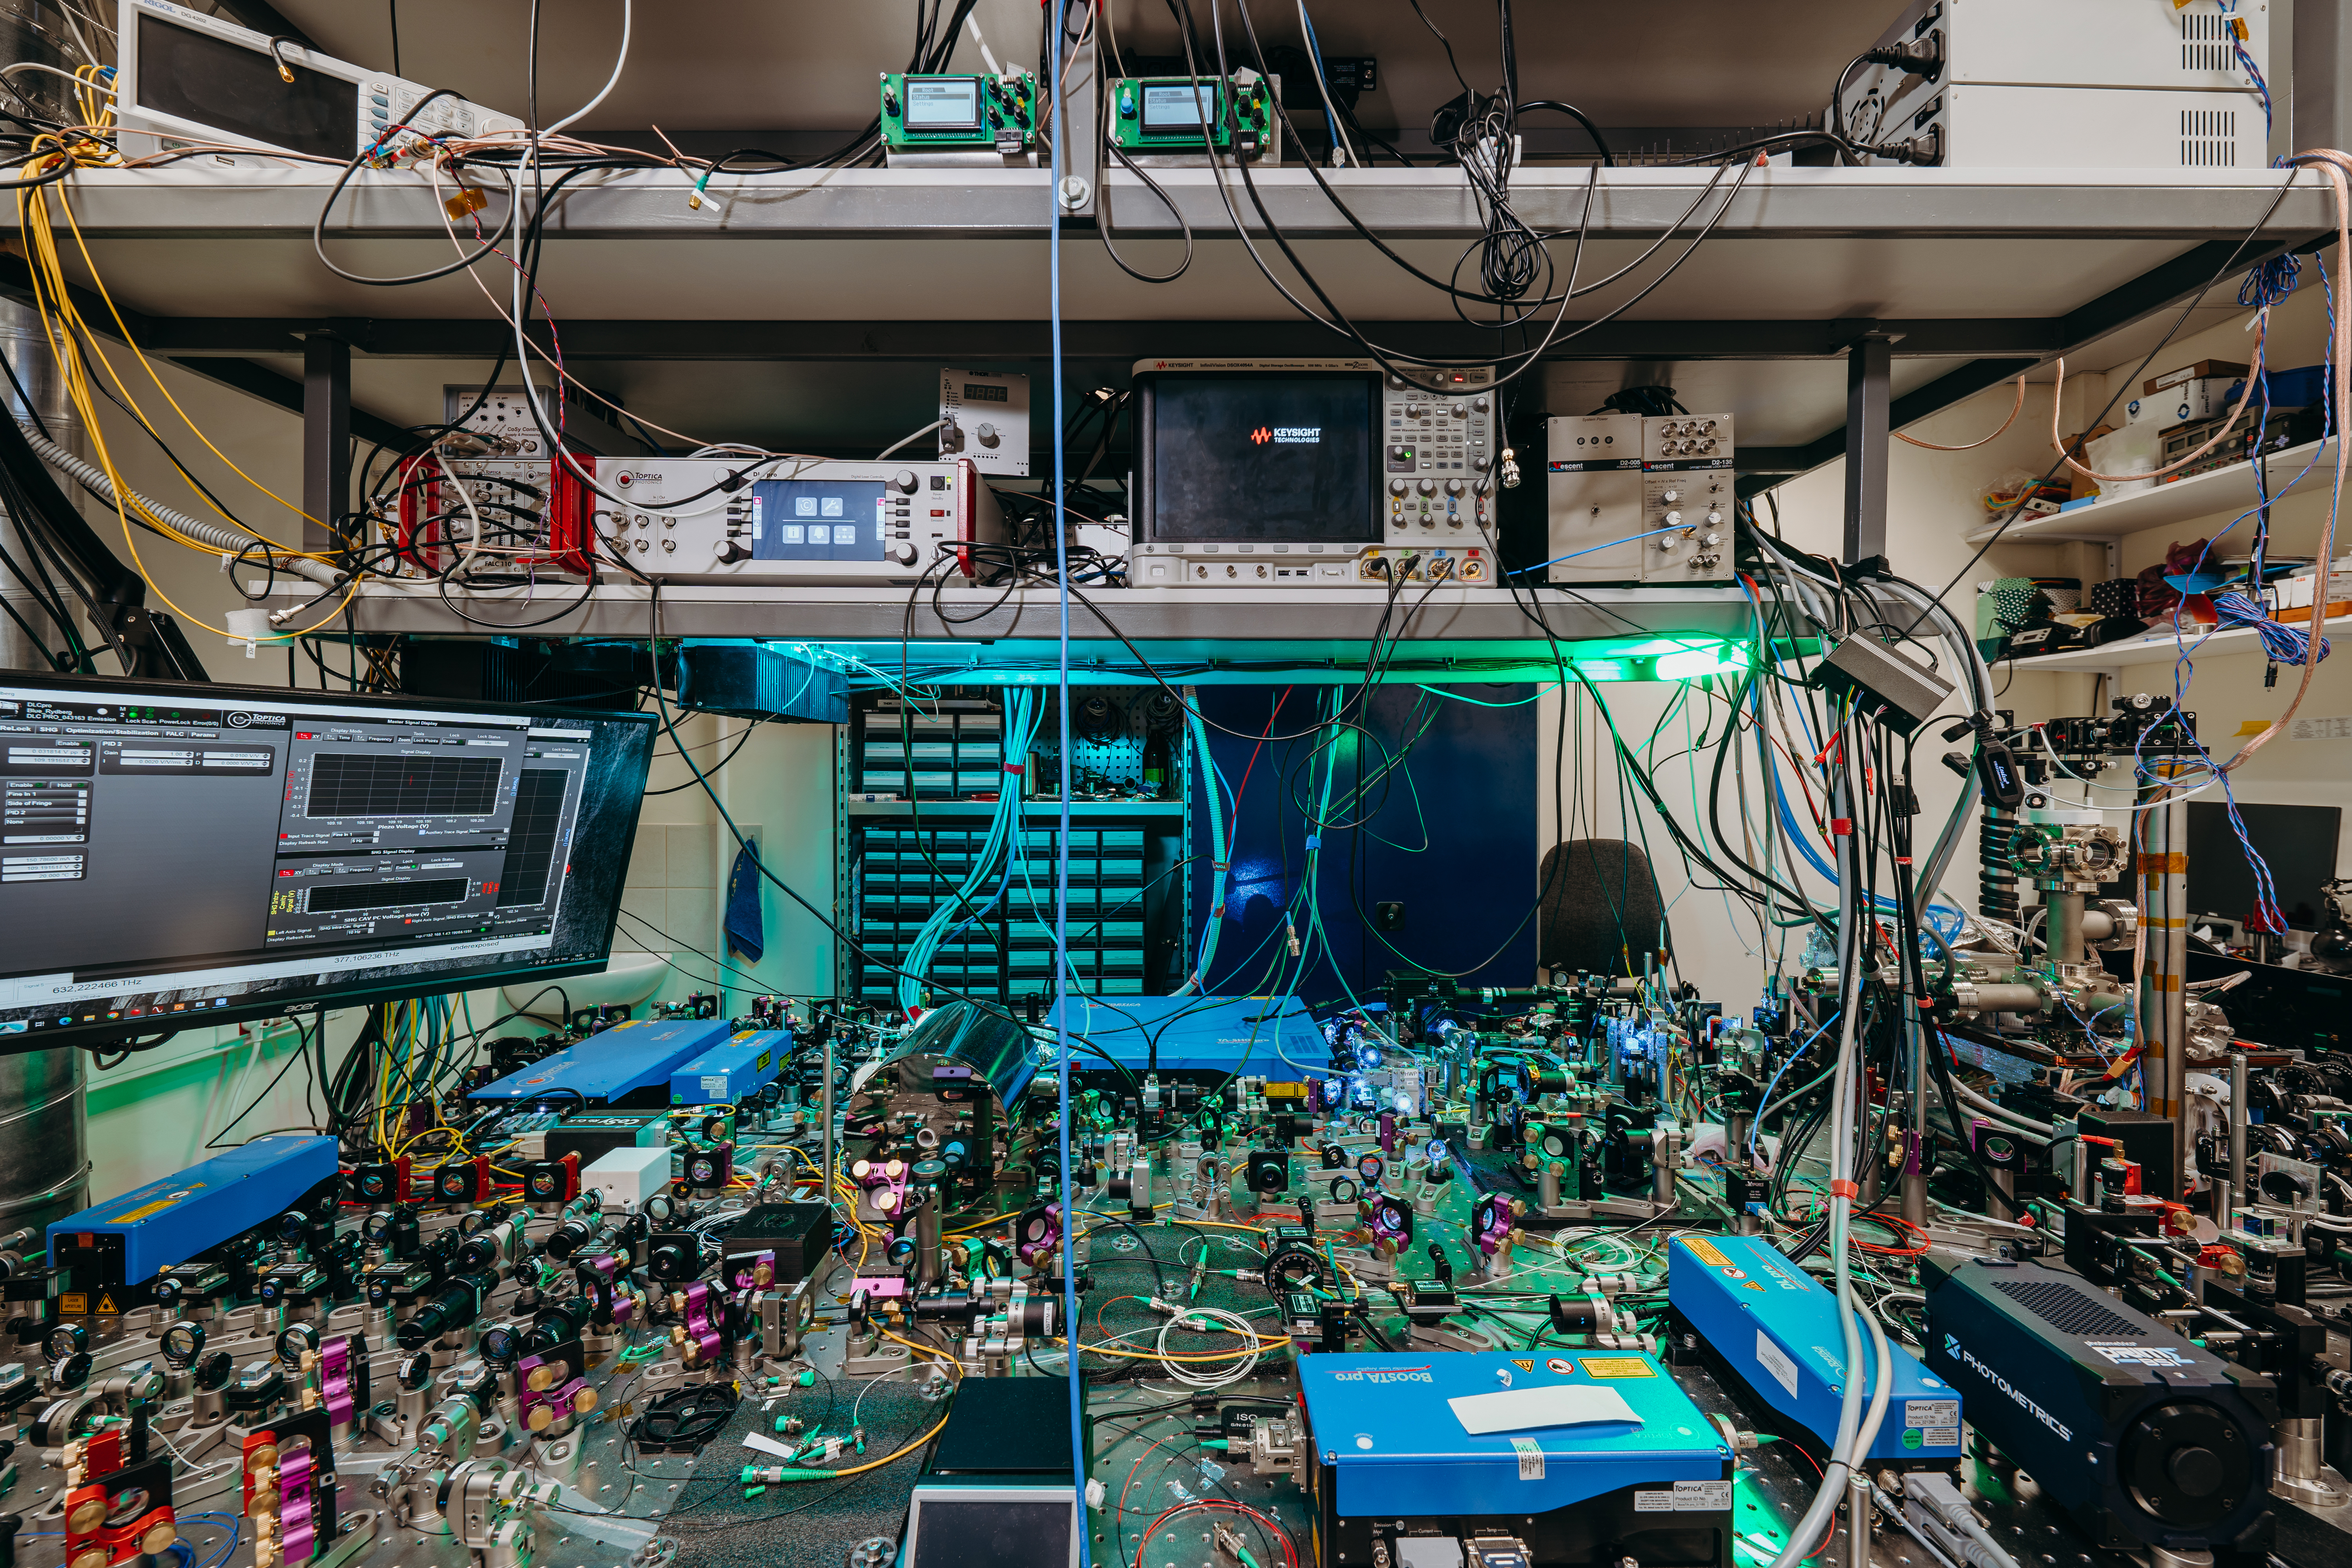
\includegraphics[width=1.0\textwidth]{images/QuantumComputer.jpg}
	\caption{Квантовый компьютер на холодных нейтральных атомах $^{87}\text{Rb}$ лаборатории ``Атомных и оптических квантовых вычислений''.}
\end{figure}

\newpage